\section{Zielsetzung}

Der vorliegende Versuch behandelt die Ermittelung der Lebensdauer
von kosmischen Myonen.

\seciton{Theorie}

Myonen $\mu$ sind Leptonen der zweiten Generation und besitzen eine Masse
von $\approx \SI{106}{\mega\eV}$.
Sie entstehen zum Großteil in der oberen Atmosphäre durch Pion-Zerfälle und
besitzen eine hohe kinetische Energie.

\begin{equation}
  \label{eqn:pion+ nach myon}
  \ce{\pi^+ -> \mu^+ + \nu\ua{\mu}}\\
  \label{eqn:pion- nach myon}
  \ce{\pi^- -> \mu^- + \bar{\nu}\ua{\mu}}
\end{equation}

\subsection{Lebensdauer}

Die Lebensdauer $\tau$ eines instabilen Teilchens beschreibt die Zeit,
nachder eine Teilchenpopulation auf $\frac{1}{\exp}$ ihrer ursprünglichen
Anzahl abgefallen ist.
Der Zerfall eines Teilchens ist ein stochastischer Prozess, der durch
ein Exponentialgesetz der Form:

\begin{equation}
  \label{eqn:Lebensdauer}
  N(t) = N_0\cdot\exp{-\frac{t}{\tau}}
\end{equation}

beschrieben wird.





\section{Durchführung}

Damit die Lebensdauer von Myonen bestimmt werden kann, dürfen nur
Myonen gemessen werden, von denen die Einlaufzeit in den Versuchsaufbau bekannt ist
und weiterhin deren Zerfallszeit nach eindringen gemessen wurde.
Somit sind nur Myonen, die auch in dem Versuchsaufbau zerfallen relevant
für die Messung. Im Folgenden wird der verwendete Versuchsaufbau beschrieben,
der das herausfiltern dieser relevanten Ereignisse ermöglicht.

Grundlegend wird für die dedektion von Teilchen ist ein Szintillator.
Geladene Teilchen, die den Szintillator durchqueren wechselwirken mit den Atomen
im Szintillatormaterial. Durch diese Wechselwirkung können
die Atome im Szintillator in einen angeregten Zustand überführen werden.
Myonen haben eine hohe kinetische Energie und können mehrere MeV ihrer kinetischen Energie
an das Szintillatormaterial abgeben. Die angeregten Szintillatoratome geben
bei dem Übergang von dem angeregten Zustand in den Grundzustand einen Lichtquant
ab, der von einer optisch an den Szintillator gekoppelten Photokathode
dedektiert werden kann.
An der Photokathodeliegt ein sekundärer Elektronenvervielfältiger (SEV) an.
Der SEV verstärkt die Signale aus der Photokathode, damit sie dedektiert werden
können.

Das Filtern der Ereignisse von Myonen, die auch in dem Szintillator zerfallen
geschieht durch eine logische Schaltung. Diese Schaltung ist in Abb. \ref{fig:Aufbau}
durch die beiden AND-Gatter und den Monoflop/Univibrator realisiert.
Anliegende Spannungen werden im Folgenden als up und das fehlen von Spannungen
als down bezeichnet.
Wenn ein up aus der Koinzidenz (vgl. Abb. \ref{fig:Aufbau}), deren Funktion im
Verlauf der Durchfürhung noch erklärt wird, in die untere Schaltung einläuft
wird zunächst der rechte Eingang des 1. und 2. UND-Gatter auf up gesetzt.
Somit sind an dem 1. UND beide Eingänge mit einem up belegt und das Startsignal wird
an einen Zeit-Amplituden-Konverter und Impulszähler gegeben. Der Impulszähler
zählt lediglich die Anzahl der eintreffenden Startsignale.
Der Zeit-Amplituden-Konverter wandelt die vergehende Zeit zwischen einem
up an dem Starteingang und einem up an dem Stopeingang in eine
dazu proportionalen Impuls. DIe Zeit wird in der Höhe des Impulses
kodiert.
Weiter zur logischen Schaltung. Das anfänglich aus der Koinzidenz stammende
up wird über eine Verzögerung von $\SI{30}{\nano\second}$   


\begin{figure}[h]
  \centering
  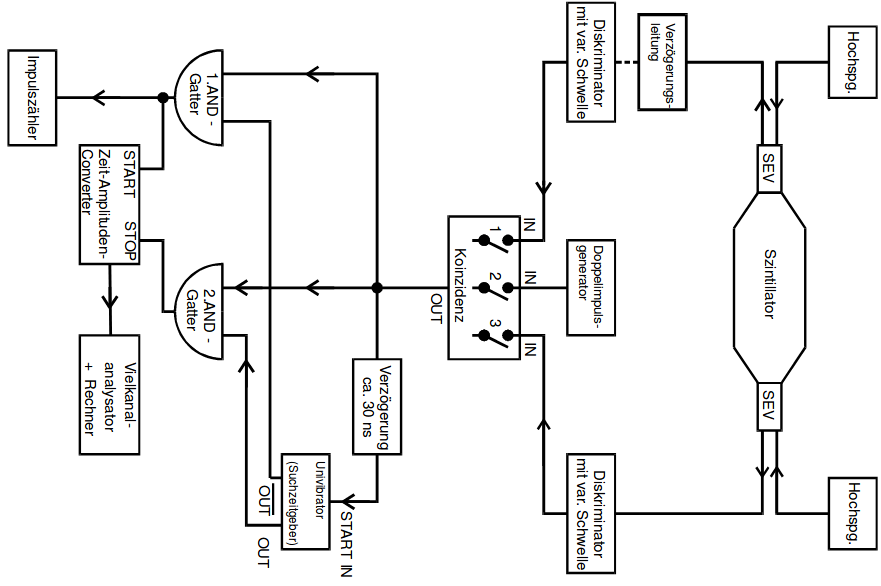
\includegraphics[width=9cm, angle=90]{Pics/Aufbau.png}
  \caption{Schematischer Versuchsaufbau \cite{anleitung01}}
  \label{fig:Aufbau}
\end{figure}

Der Versuch wird mit dem Aufbau aus Abb. \ref{fig:Aufbau} durchgeführt. In
dem realen Aufbau ist ein weiterer Verzögerer vor dem rechten Diskriminator angebracht,
sodass eine Verzögerung der beiden Messkanäle relativ zu einander eingestellt werden kann.

In dem Versuch wird ein organischer Szintillator verwendet, da dieser
im Vergleich zu einem anorganischen Szintillator eine kürzere
Totzeit besitzt. Insgesamt fasst der Szintillator 50l und ist mit Toluol befüllt.
